\newcommand{\brgc}[1]{%
    \begin{tabular}{cccccccc}
        0&0&0&0&1&1&1&1 \\
        0&0&1&1&1&1&0&0 \\
        0&1&1&0&0&1&1&0 \\
        \textbf{#1}&\textbf{#1}&\textbf{#1}&\textbf{#1}&\textbf{#1}&\textbf{#1}&\textbf{#1}&\textbf{#1} 
    \end{tabular}%
}
\newcommand{\brgcinv}[1]{%
    \begin{tabular}{cccccccc}
        1&1&1&1&0&0&0&0 \\
        0&0&1&1&1&1&0&0 \\
        0&1&1&0&0&1&1&0 \\
        \textbf{#1}&\textbf{#1}&\textbf{#1}&\textbf{#1}&\textbf{#1}&\textbf{#1}&\textbf{#1}&\textbf{#1} 
    \end{tabular}%
}

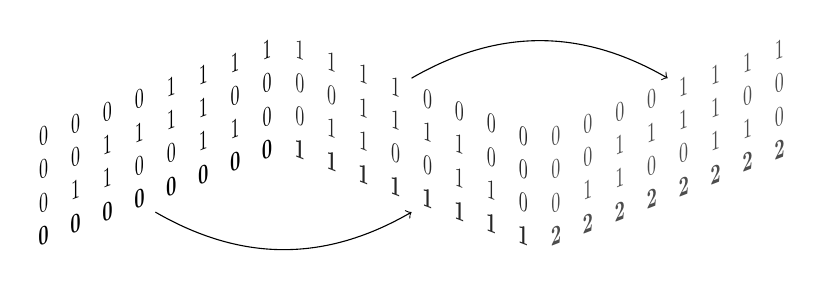
\begin{tikzpicture}

    % 1. The first copy (Slanting UPWARDS)
    \begin{scope}[xscale=0.65, yslant=0.25, transform shape]
        \node[anchor=west, inner sep=0pt] (panel1) at (0,0) {\brgc{0}};
    \end{scope}
    
    % 2. The second copy (Slanting DOWNWARDS)
    % Attaches to the right edge of panel 1
    \begin{scope}[xscale=0.65, yslant=-0.25, transform shape]
        \node[anchor=west, inner sep=0pt, opacity=0.85] (panel2) at (panel1.east) {\brgcinv{1}};
    \end{scope}

    % 3. The third copy (Slanting UPWARDS again)
    % Attaches to the right edge of panel 2
    \begin{scope}[xscale=0.65, yslant=0.25, transform shape]
        \node[anchor=west, inner sep=0pt, opacity=0.7] (panel3) at (panel2.east) {\brgc{2}};
    \end{scope}

    \draw[->] (panel1.south) to[bend right] (panel2.south);
    \draw[->] (panel2.north) to[bend left] (panel3.north);

\end{tikzpicture}